\chapter{Backend} \label{chap:backend}

%Two basic transfer functions are shown in \cref{fig:methods:transfer_functions}.

%\begin{figure}[H]
%  \centering
%  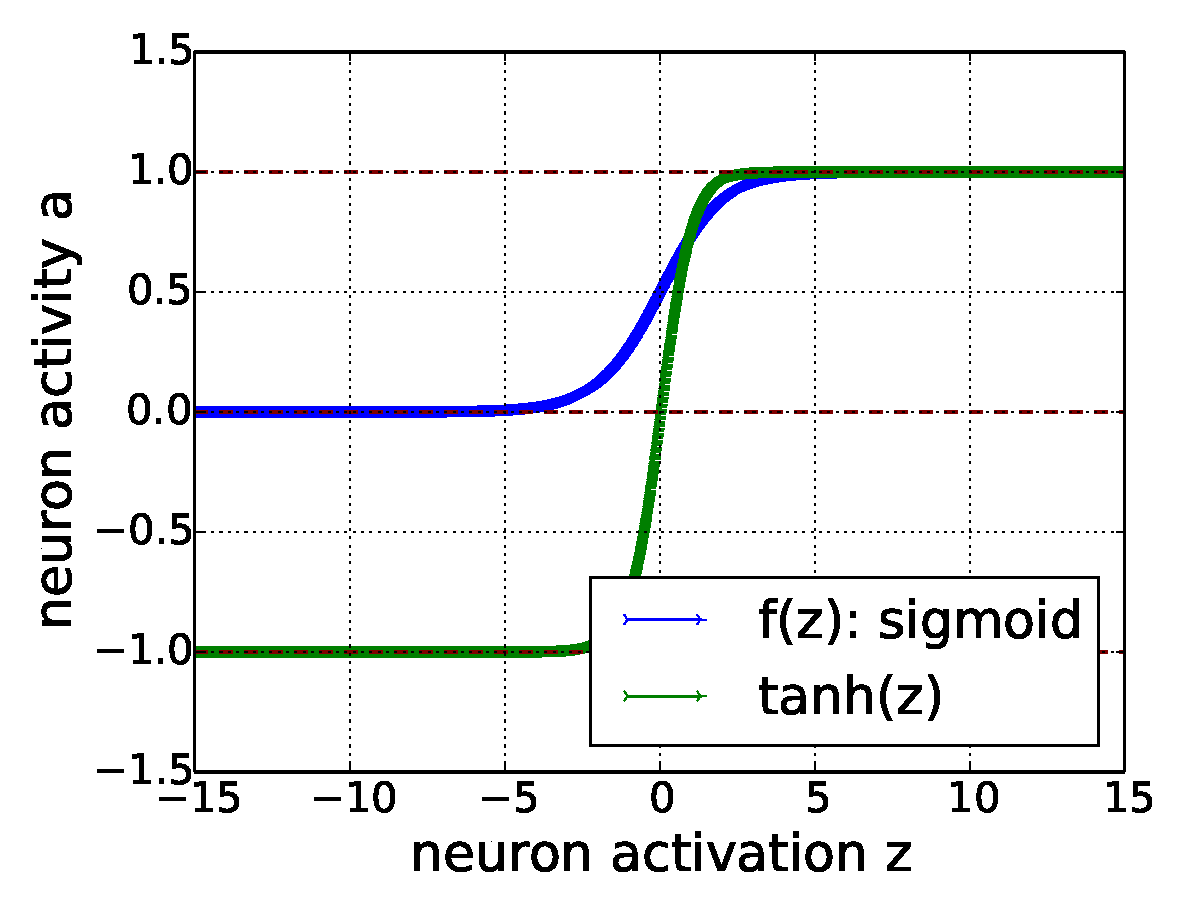
\includegraphics[width=0.7\textwidth]{transfer_functions.eps}
%  \caption{Transfer functions: \textit{Sigmoid} and \textit{Tanh}}
%  \label{fig:methods:transfer_functions}
%\end{figure}

Own engine running on Raspberry Pi 4 has been developed and serves as the backend for the project. The whole engine is coded in Python, and adheres to the following principles:
\begin{itemize}
	\item \textit{Simplicity}: write a straightforward code that is easily understandable for later rewriting.
	\item \textit{Modifiability}: write a code with the ability to admit changes due to a new requirement or detect an error that needs to be fixed.
	\item \textit{Modularity}: write a well-encapsulated code of modules, which do particular, well-documented functions.
	\item \textit{Robustness}: write a code focusing on handling unexpected termination and unexpected actions.
\end{itemize}
%https://www.pharmasug.org/proceedings/2011/TT/PharmaSUG-2011-TT05.pdf


\section{Diagram description} \label{section:diagram description}

This section briefly describes the architecture of the engine that is figured on a diagram - see  \cref{fig:vh_project_design}.

\begin{figure}[H]
  \centering
  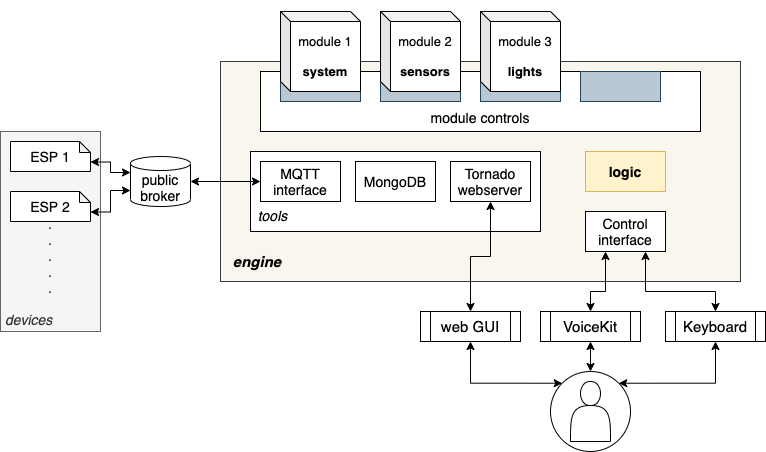
\includegraphics[width=0.85\textwidth]{img/vh_project_design.png}
  \caption{Project architecture}
  \label{fig:vh_project_design}
\end{figure}

Engine uses tools like MQTT, MongoDB, Tornado web server that is described later. Each of them runs in its thread and concurrently. These tools create a basis for modules and mediate main functionalities such as database, web server and communication. 

The engine is designed to easily remove, add or update any mutually independent modules that define functions used by a user interface. Each module is described in the \cref{chap:modules}.

The engine also contains a separate block for \textit{logic}. This block captures a command from the VoiceKit or keyboard interface, then browsing a predefined list of each module's commands and determines the best match for the user voice command or command written on the keyboard. If it does not find the voice command in lists, it replies that the command has not found with the recognized command.

\section{Database} \label{section:database}


% An auxiliary database is needed to store all the sensors data. For this purpose, MongoDB is used due to the following advantages. 

MongoDB is an open-source document database built upon a NoSQL database and written in C++. Database's horizontal, scale-out architecture support vast volumes of both data and traffic. One document can have others embedded in itself, and there is no need to declare the structure of documents to the system - documents are self-describing.\citep{mongoDB_jayaram_2020}

Before using this type of database, we have to be familiar with different terminology compare to traditional SQL databases: 
\begin{table}[H]
	\centering
	\begin{tabular}{|l|l|} \hline
		SQL Server & MongoDB \\ \hline\hline
		Database & Database \\ \hline
		Table & Collection \\ \hline
		Index & Index \\ \hline
		Row & Document \\ \hline
		Column & Field \\ \hline
		Joining & Linking \& Embedding \\ \hline
		Partition & Sharding (Range Partition) \\ \hline
		Replication & ReplSet\\ \hline
	\end{tabular}
	\caption{MongoDB terminology}
	\label{tab:mongoDB_terminology}
\end{table}

We use this type of database because it is famous for its use in agile methodologies, and the project tends to enlarge in the future. The main benefits are:
\begin{itemize}
	\item MongoDB is easy to scale.
	\item Schema-less database: we do not need to design the database's schema because the code we write defines the schema, thus saves much time.
	\item The document query language supported by MongoDB is simplistic as compared to SQL queries.
	\item There is no need for mapping application's objects to database's objects in MongoDB.
	\item No complex joins are needed in MongoDB. There is no relationship among data in MongoDB.
	\item Because of using JSON\footnote{\textbf{J}ava\textbf{S}cript \textbf{O}bject \textbf{N}otation} format to store data, it is effortless to store arrays and objects.
	\item MongoDB is free to use. There is no cost for it.
	\item MongoDB is simple to set up and install.
\end{itemize}

For adding a new field, the field can be created without affecting all other documents in the collection, without updating a central system catalog, and without taking the system offline. 

In the project, we save all incoming messages from MQTT to MongoDB to a collection based on a name of interest module.

\section{Communication}

Communication is the backbone of the whole project among several devices over the internet. Therefore, it had to be found robust, scalable, and cost-effective protocols that transmit messages and data securely.Based on the survey, we choose three protocols that, in combination, satisfy all our requirements, and we will delve deeper into them in the following sections.

\subsection{MQTT}

MQTT is a standardized protocol by the OASIS MQTT Technical Committee used for message and data exchange. The protocol is designed specifically for the Internet of Things. The protocol is developed in vast language diversity from low-level to high-level programming language and designed at light versions for low-performance devices. Hence, it suits our use-case perfectly because each module possesses tons of various devices with limited resources that are already included or will arise later on. \citep{mqtt_malý_2016}

\begin{figure}[H]
	\centering
	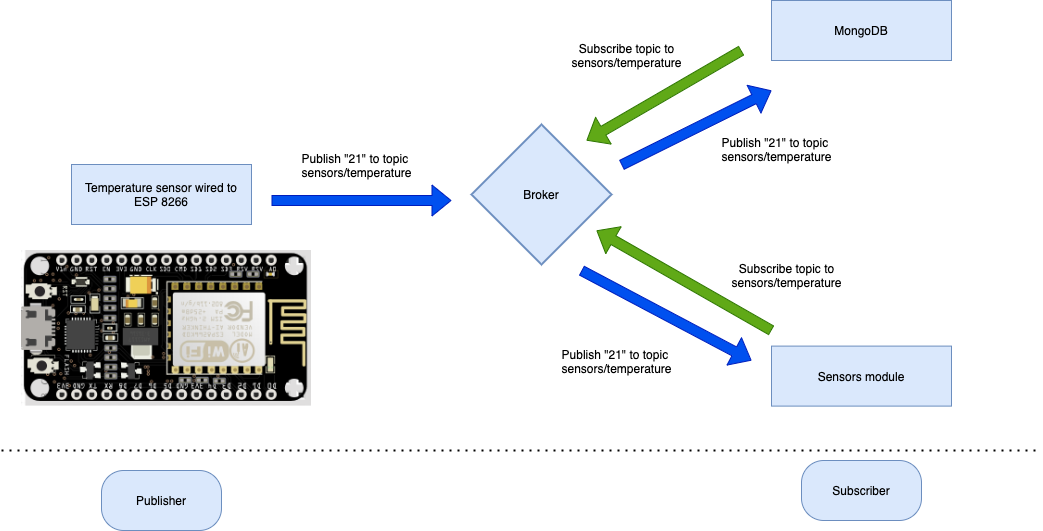
\includegraphics[width=\textwidth]{img/MQTT_pub_sub_pattern.png}
	\caption{MQTT publisher/subscriber pattern}
	\label{fig:MQTT_pub_sub_pattern}
  \end{figure}

The design principles are to minimize network bandwidth and device resource requirements whilst also attempting to ensure reliability and some degree of assurance of delivery. The protocol determines errors by TCP and orchestrates communication by the central point - broker. The protocol architecture uses a publish/subscribe pattern (also known as pub/sub) shown in \cref{fig:MQTT_pub_sub_pattern}, which provides an alternative to traditional client-server architecture. Architecture decouples publishers and subscribers who never contact each other directly and are not even aware that the other exist. The decoupling give us the following advantage:

\begin{itemize}
	\item \textit{Space decoupling}: publisher and subscriber do not need to know each other.
	\item \textit{Time decoupling}: publisher and subscriber do not need to run at the same time.
	\item \textit{Synchronization decoupling}: operations on both components do not need to be interrupted during publishing or receiving.
\end{itemize}

When the publisher sends his message, it is handled by the broker who filters all incoming messages and distributes them to accredited subscribers. The filtering is based on topic or subject, content and type.

In the case of MQTT, the filtering is subject-based and therefore, every message including a subject or a topic. The client subscribes to the topics he is interested in, and the broker distributes the messages accordingly as shown in \cref{fig:MQTT_pub_sub_communication_diagram}.

\begin{figure}[H]
	\centering
	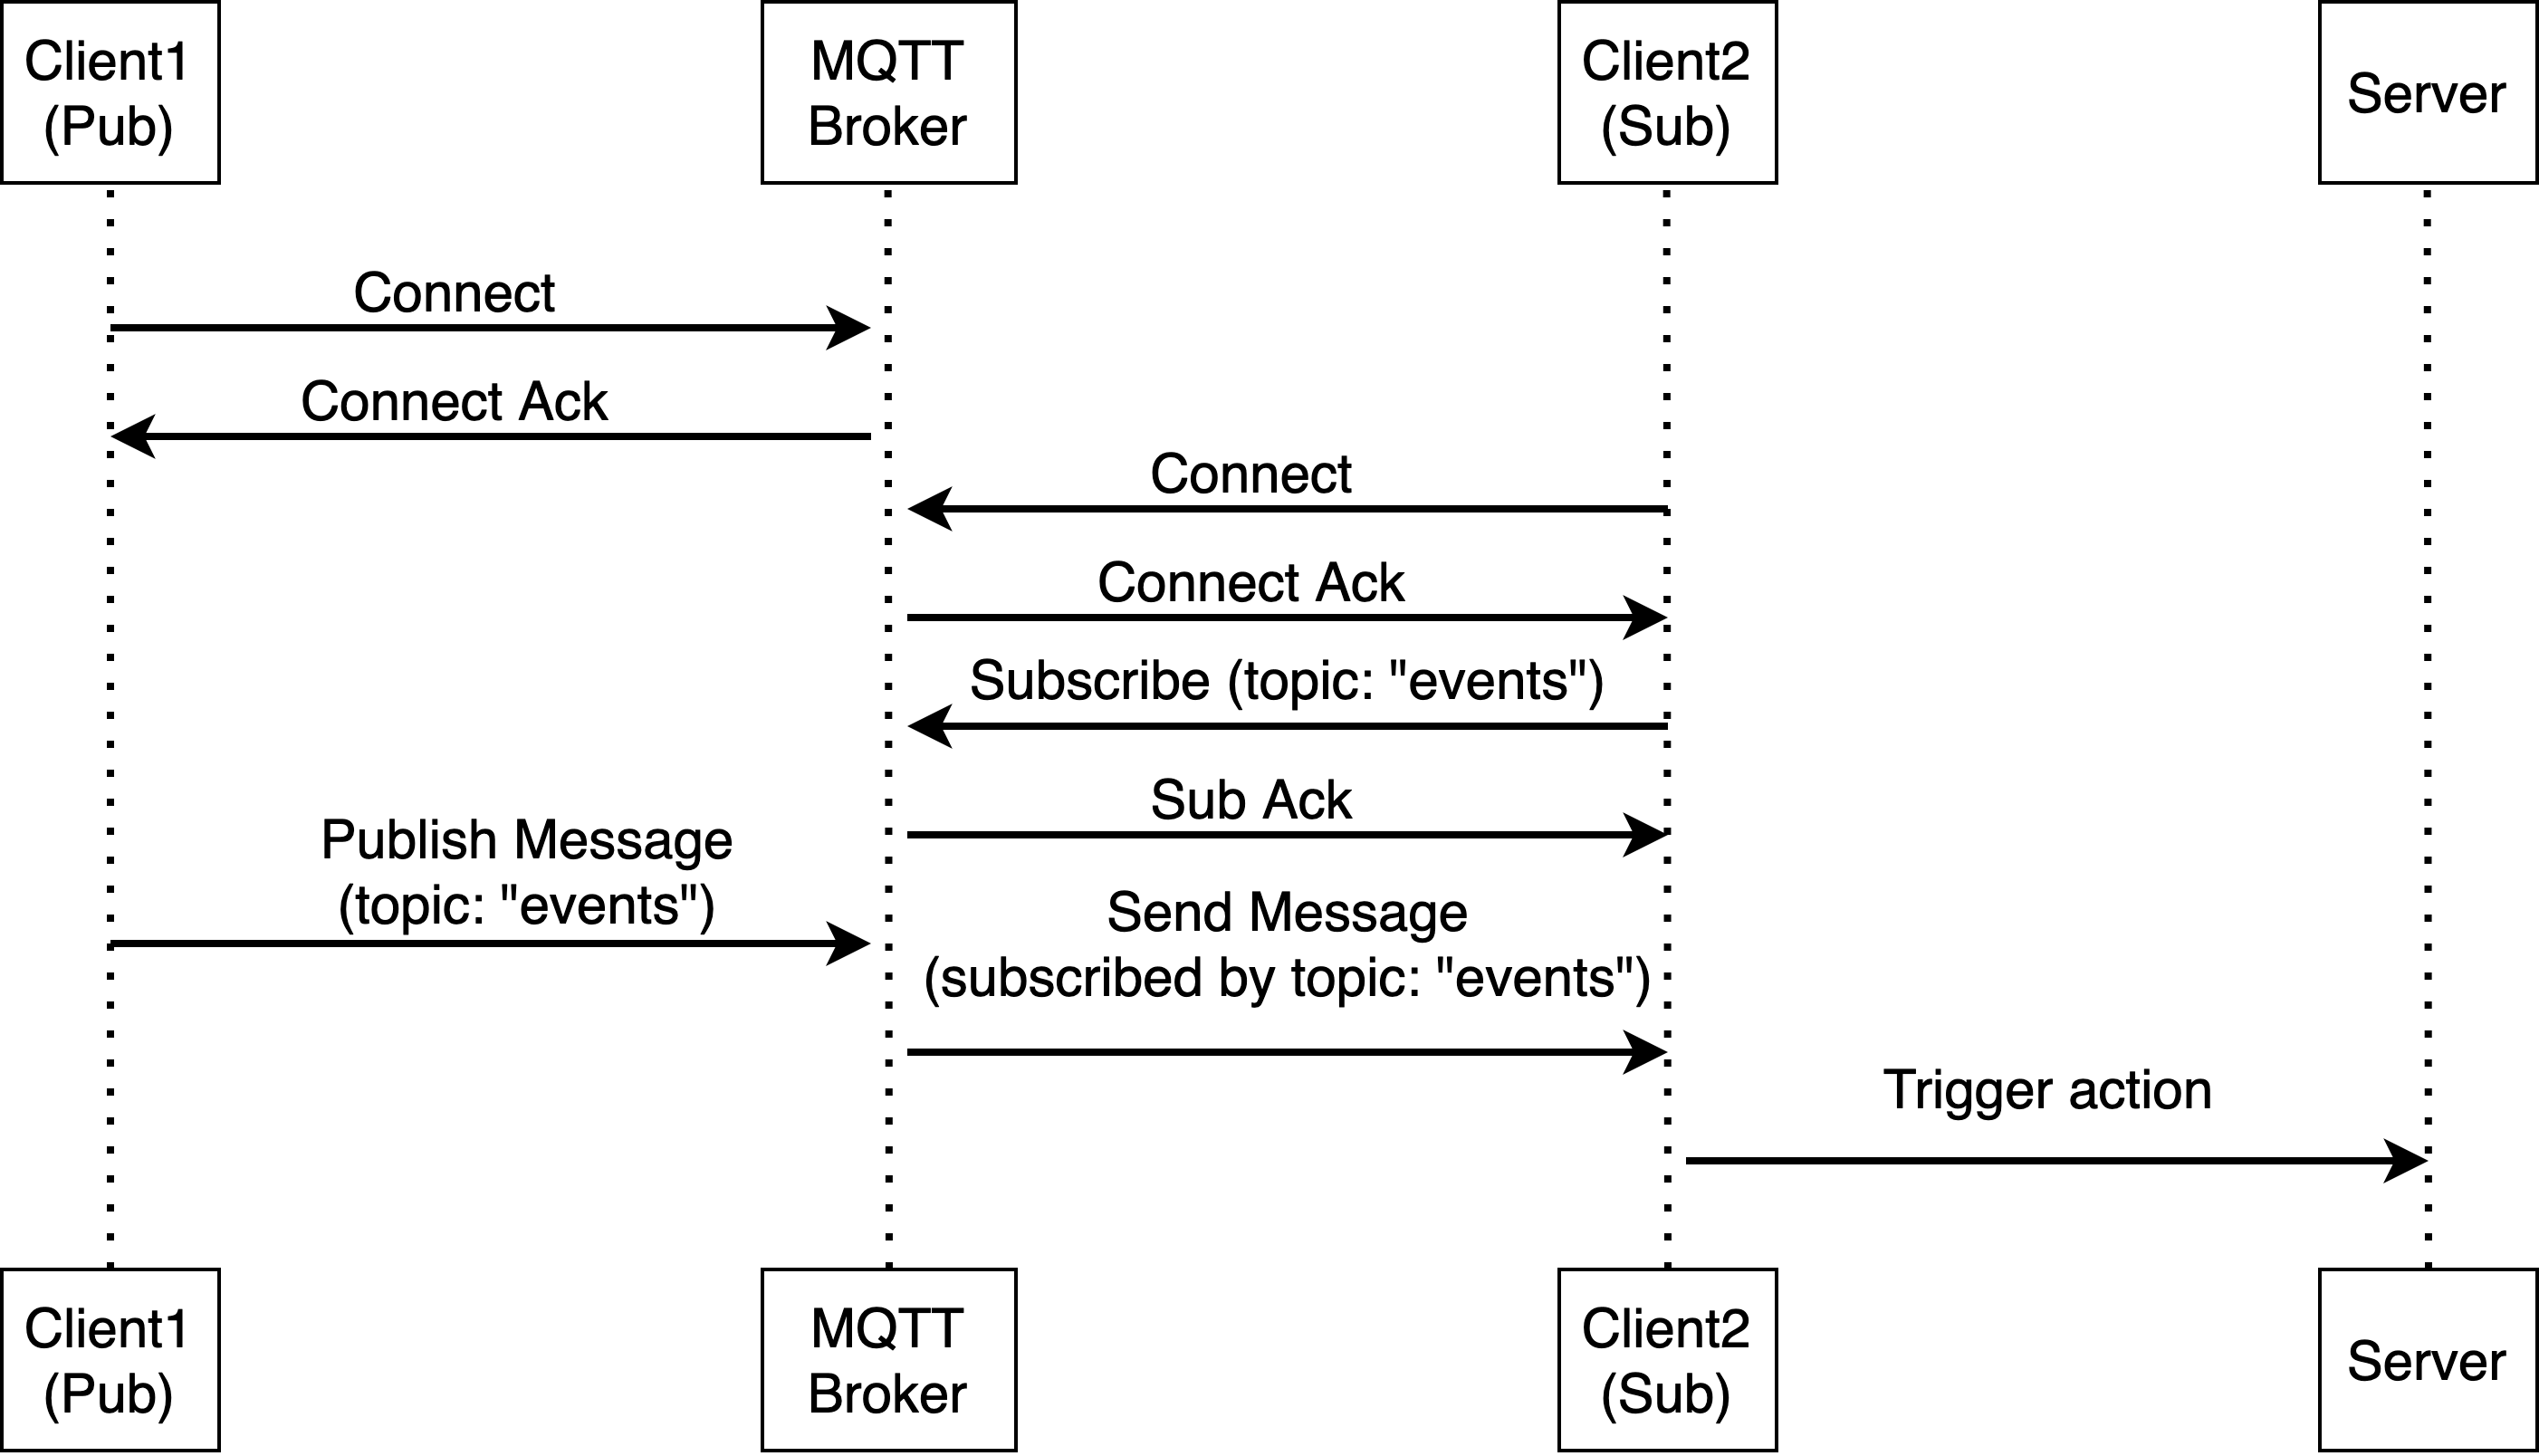
\includegraphics[width=\textwidth]{img/MQTT_pub_sub_communication_diagram.png}
	\caption{Diagram illustrating how communication in MQTT flow.}
	\label{fig:MQTT_pub_sub_communication_diagram}
  \end{figure}

The topics are generally strings with a hierarchical structure that allow different subscription levels. It is feasible to use wildcards to subscribe, for example, sensors/\# to receive all messages related to the sensors, for example, sensors/temperature or sensors/illuminance.

The MQTT protocol has the Quality of Service (QoS) levels essential to any communication protocol.  The level of QoS can be specified for each message or topic separately according to its importance.

In MQTT, there are 3 QoS levels:

\begin{itemize}
	\item \textit{QoS 0}: This level is often called "fire and forget" when a message is not stored and retransmitted by a sender.
	\item \textit{QoS 1}: Is is guarantees that a message is delivered at least one time to the receiver. The message is stored on a sender until it gets a PUBACK packet from a receiver.
	\item \textit{QoS 2}: It is the highest level, and it guarantees that each message received only once by the intended recipients.
\end{itemize}

It is vital to mention MQTT have the feature retained messages that are mechanisms where the broker stores the last retained message for a specific topic. This feature allows a client does not have to wait until a new message is published to know the last known status of other devices.
 
\subsection{WebSocket}
 
In this work, WebSockets are used to provide communication between the client and the engine. WebSocket provides a low-latency, persistent, full-duplex connection between a client and server over TCP. The protocol is chiefly used for a real-time web application because it is faster than HTTP concerning more transfers by one connection. The protocol belongs to the stateful type of protocols, which means the connection between client and server will keep alive until either client or web server terminate it. The protocol fits for us in use between client and web server in case of real-time response.\citep{websocket_wang_salim_moskovits_2013}

The main benefits are:

\begin{itemize}
	\item \textit{Persistent}: After an initial HTTP handshake, the connection keeps alive using a ping-pong process, in which the server continuously pings the client for a response. It is a more efficient way than establishing and terminating the connection for each client request and server response. Server terminating connection after an explicit request from the client, or implicitly when the client goes offline.
	\item \textit{Secure}: WebSocket Secure uses standard SSL and TLS encryption to establish a secure connection. Although we do not pursue this issue in our work, it is a valuable feature to add later.
	\item \textit{Extensible}: Protocol is designed to enabling the implementation of subprotocols and extensions of additional functionality such as MQTT, WAMP, XMPP\footnote{E\textbf{x}tensible \textbf{M}essaging and \textbf{P}resence \textbf{P}rotocol - messaging and presence protocol based on XML and mainly used in a near-real-time exchange of structured data.}, AMQP\footnote{\textbf{A}dvanced \textbf{M}essage \textbf{Q}ueuing \textbf{P}rotocol - an open standard application layer protocol for message-oriented middleware.}, multiplexing and data compression. This benefit makes WebSockets a future-proof solution for the possible addition of other functionalities.
	\item \textit{Low-latency}: WebSocket significantly reduces each message's data size, drastically decreasing latency by eliminating the need for a new connection with every request and the fact that after the initial handshake, all subsequent messages include only relevant information.
	\item \textit{Bidirectional} - This enables the engine to send real-time updates asynchronously, without requiring the client to submit a request each time, as is the case with HTTP. 
\end{itemize}

We will apply this protocol for transfer between clients such as VoiceKit, keyboard or web interface and engine in case of real-time response.

\subsection{REST}

In other cases like fetching data only once or data that is not required very frequently, we use RESTfull web service on a web server. This service enables us to transfer a lightweight data-interchange format JSON trivially and reliably - see \cref{fig:REST_schema}. We use a standard GET REST request on a defined URI and then decode it like JSON for fetching data.

\begin{figure}[H]
  \centering
  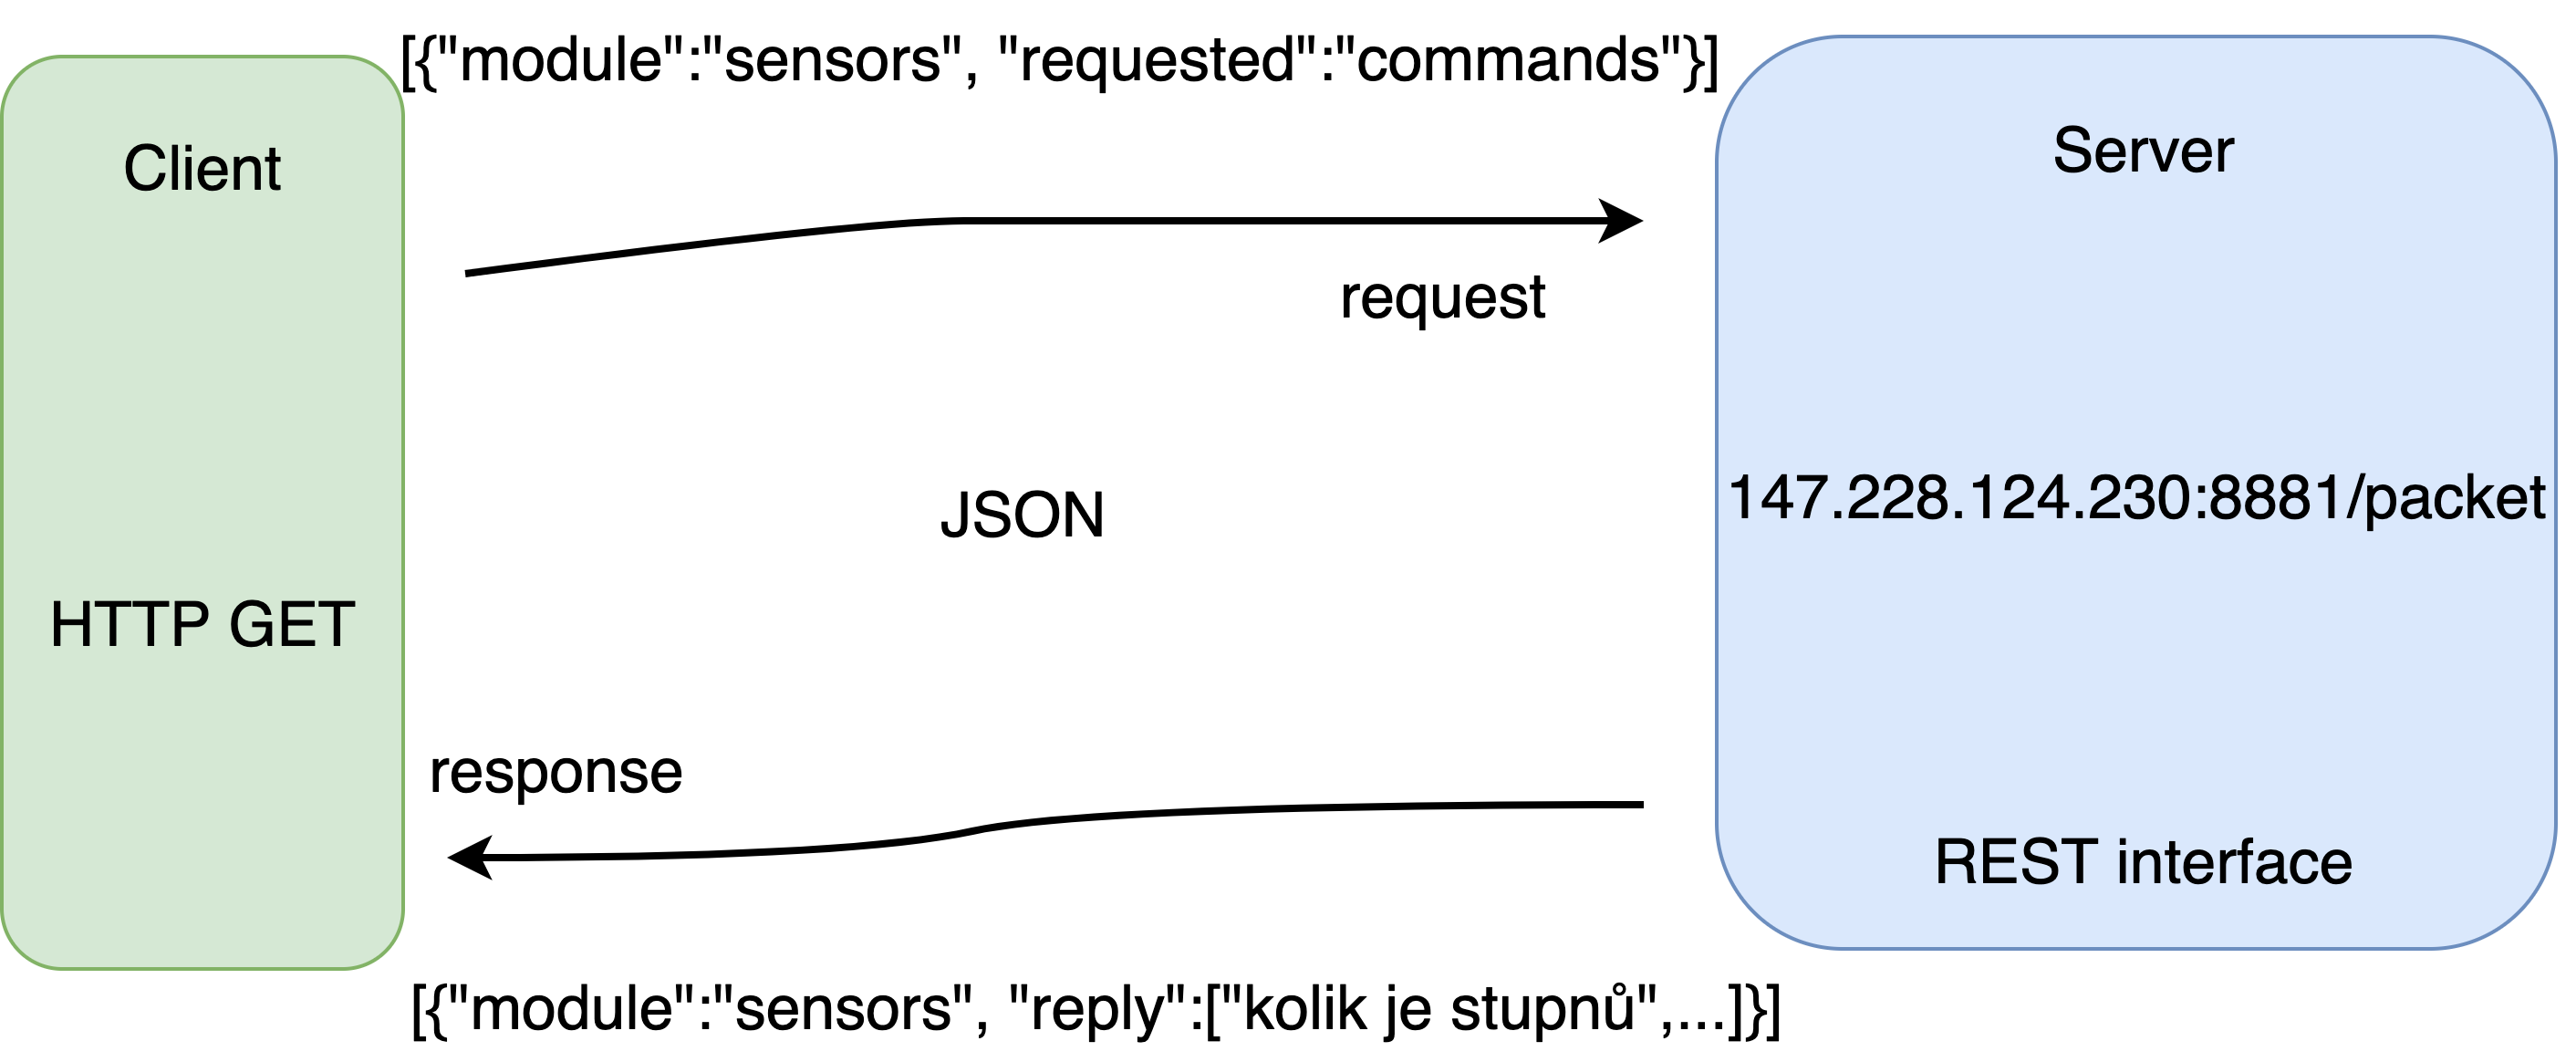
\includegraphics[width=\textwidth]{img/REST_schema.png}
  \caption{REST principle}
  \label{fig:REST_schema}
\end{figure}

\section{Controllers}

\subsection{Keyboard}

The keyboard is a python script with a particular purpose for developing new voice commands. This script opens up a CLI built upon a voicehome controller. The developer can quickly type a voice command with high accuracy through the command-line and debug the command thoroughly in various forms.

\subsection{VoiceKit}

VoiceKit is a building kit made by Google that lets users create their natural language processor and connect it to the Google Assistant or Cloud Speech-to-Text service. By pressing a button on top, users can ask questions and issue voice commands to their programs. All of this fits in a handy little cardboard cube powered by a Raspberry Pi.\citep{aiy_projects}

\begin{figure}[H]
	\centering
	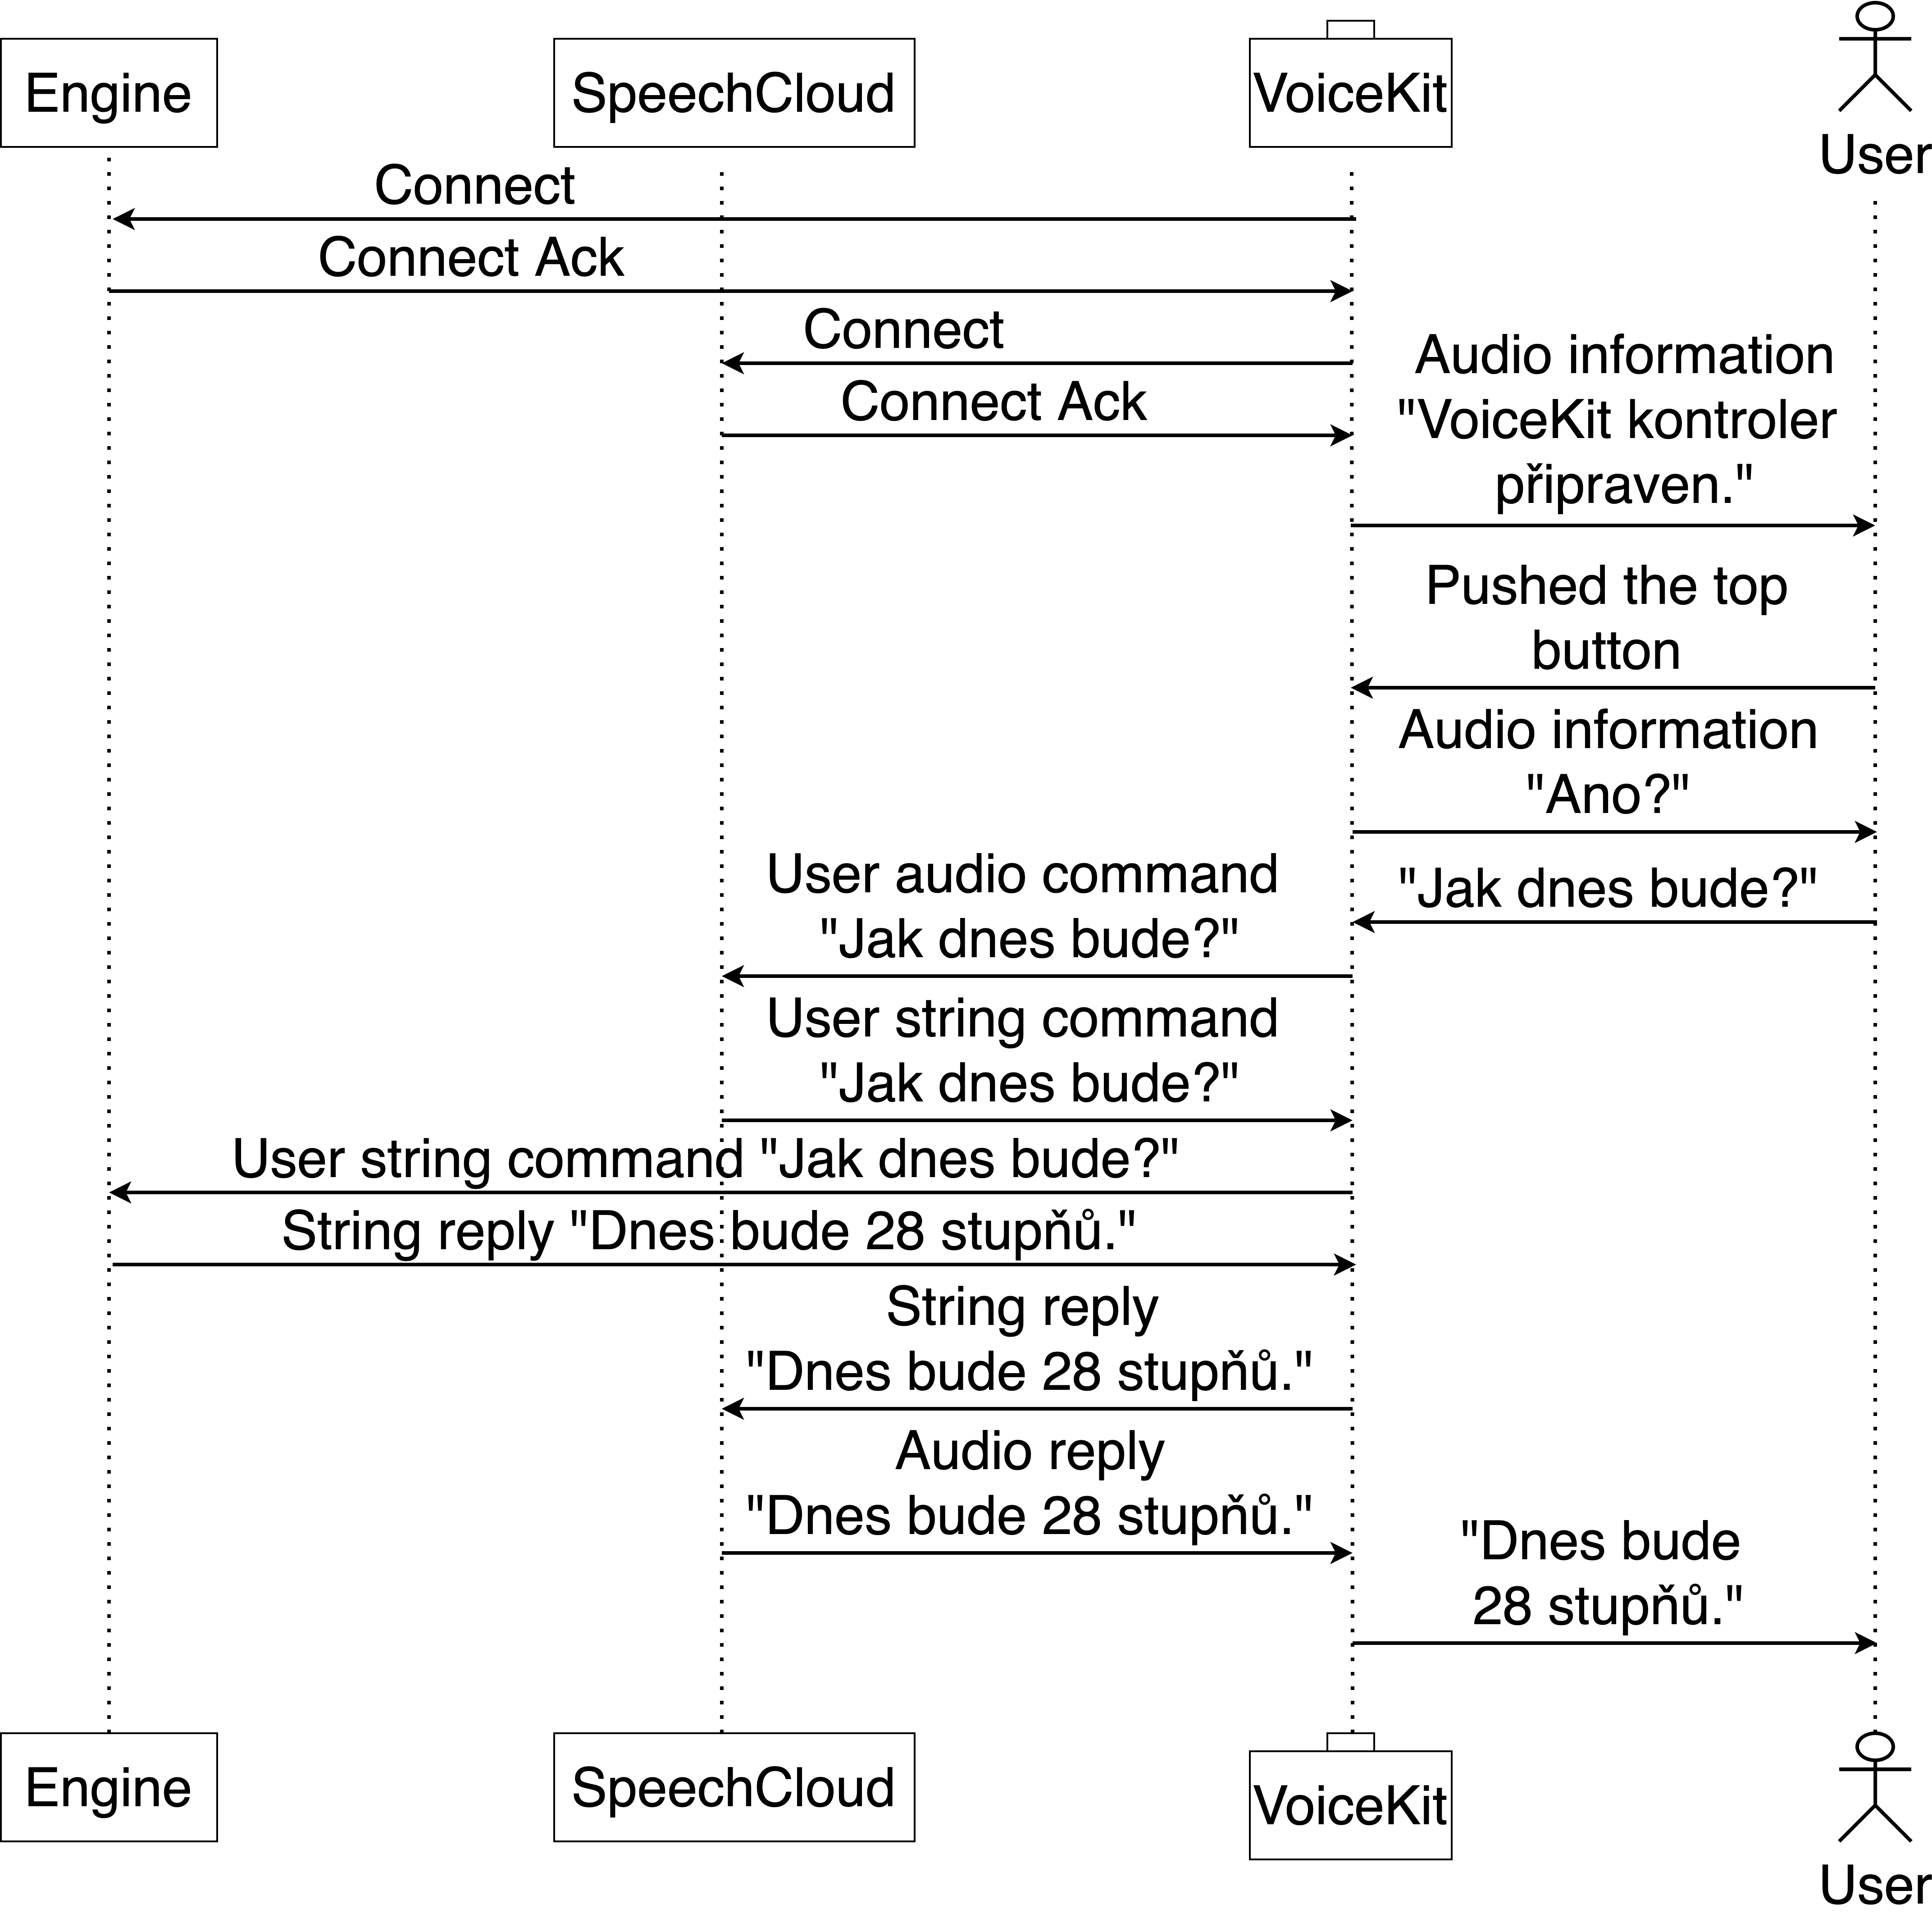
\includegraphics[width=\textwidth]{img/message_flow.png}
	\caption{Diagram of messages flows during a conversation}
	\label{fig:message_flow}
\end{figure}

\cref{fig:message_flow} show a diagram of messages flows during a conversation. It is evident from the diagram that all communication with a user and the SpeechCloud mediate VoiceKit thus engine can manipulate just with a text.

\subsection{Website}

As the second interface next to the already mentioned Voice Kit is a website. The web server is implemented in Python using the Tornado framework.

The website's architecture aims to use it via a portable device like a smartphone and tablet or touch screen attached to the wall. Therefore the website is constructed to be responsible, straightforward and touch-friendly. The website's use-cases are to able the user to monitor ESP, sensors, lights, weather and voice commands, display historical sensors data, feasible voice commands and description of them, trigger lights and modules.

The website communicates with the engine by the already mentioned WebSocket. Figure \ref{fig:lights_onoff_messages} show an example of communication between the web site and the ESP to turn on an onboard led. Communication uses JSON as a data format and is evident from the figure that web site and engine use for communicating protocol WebSocket, whereas ESP and engine use MQTT.

\begin{figure}[H]
	\centering
	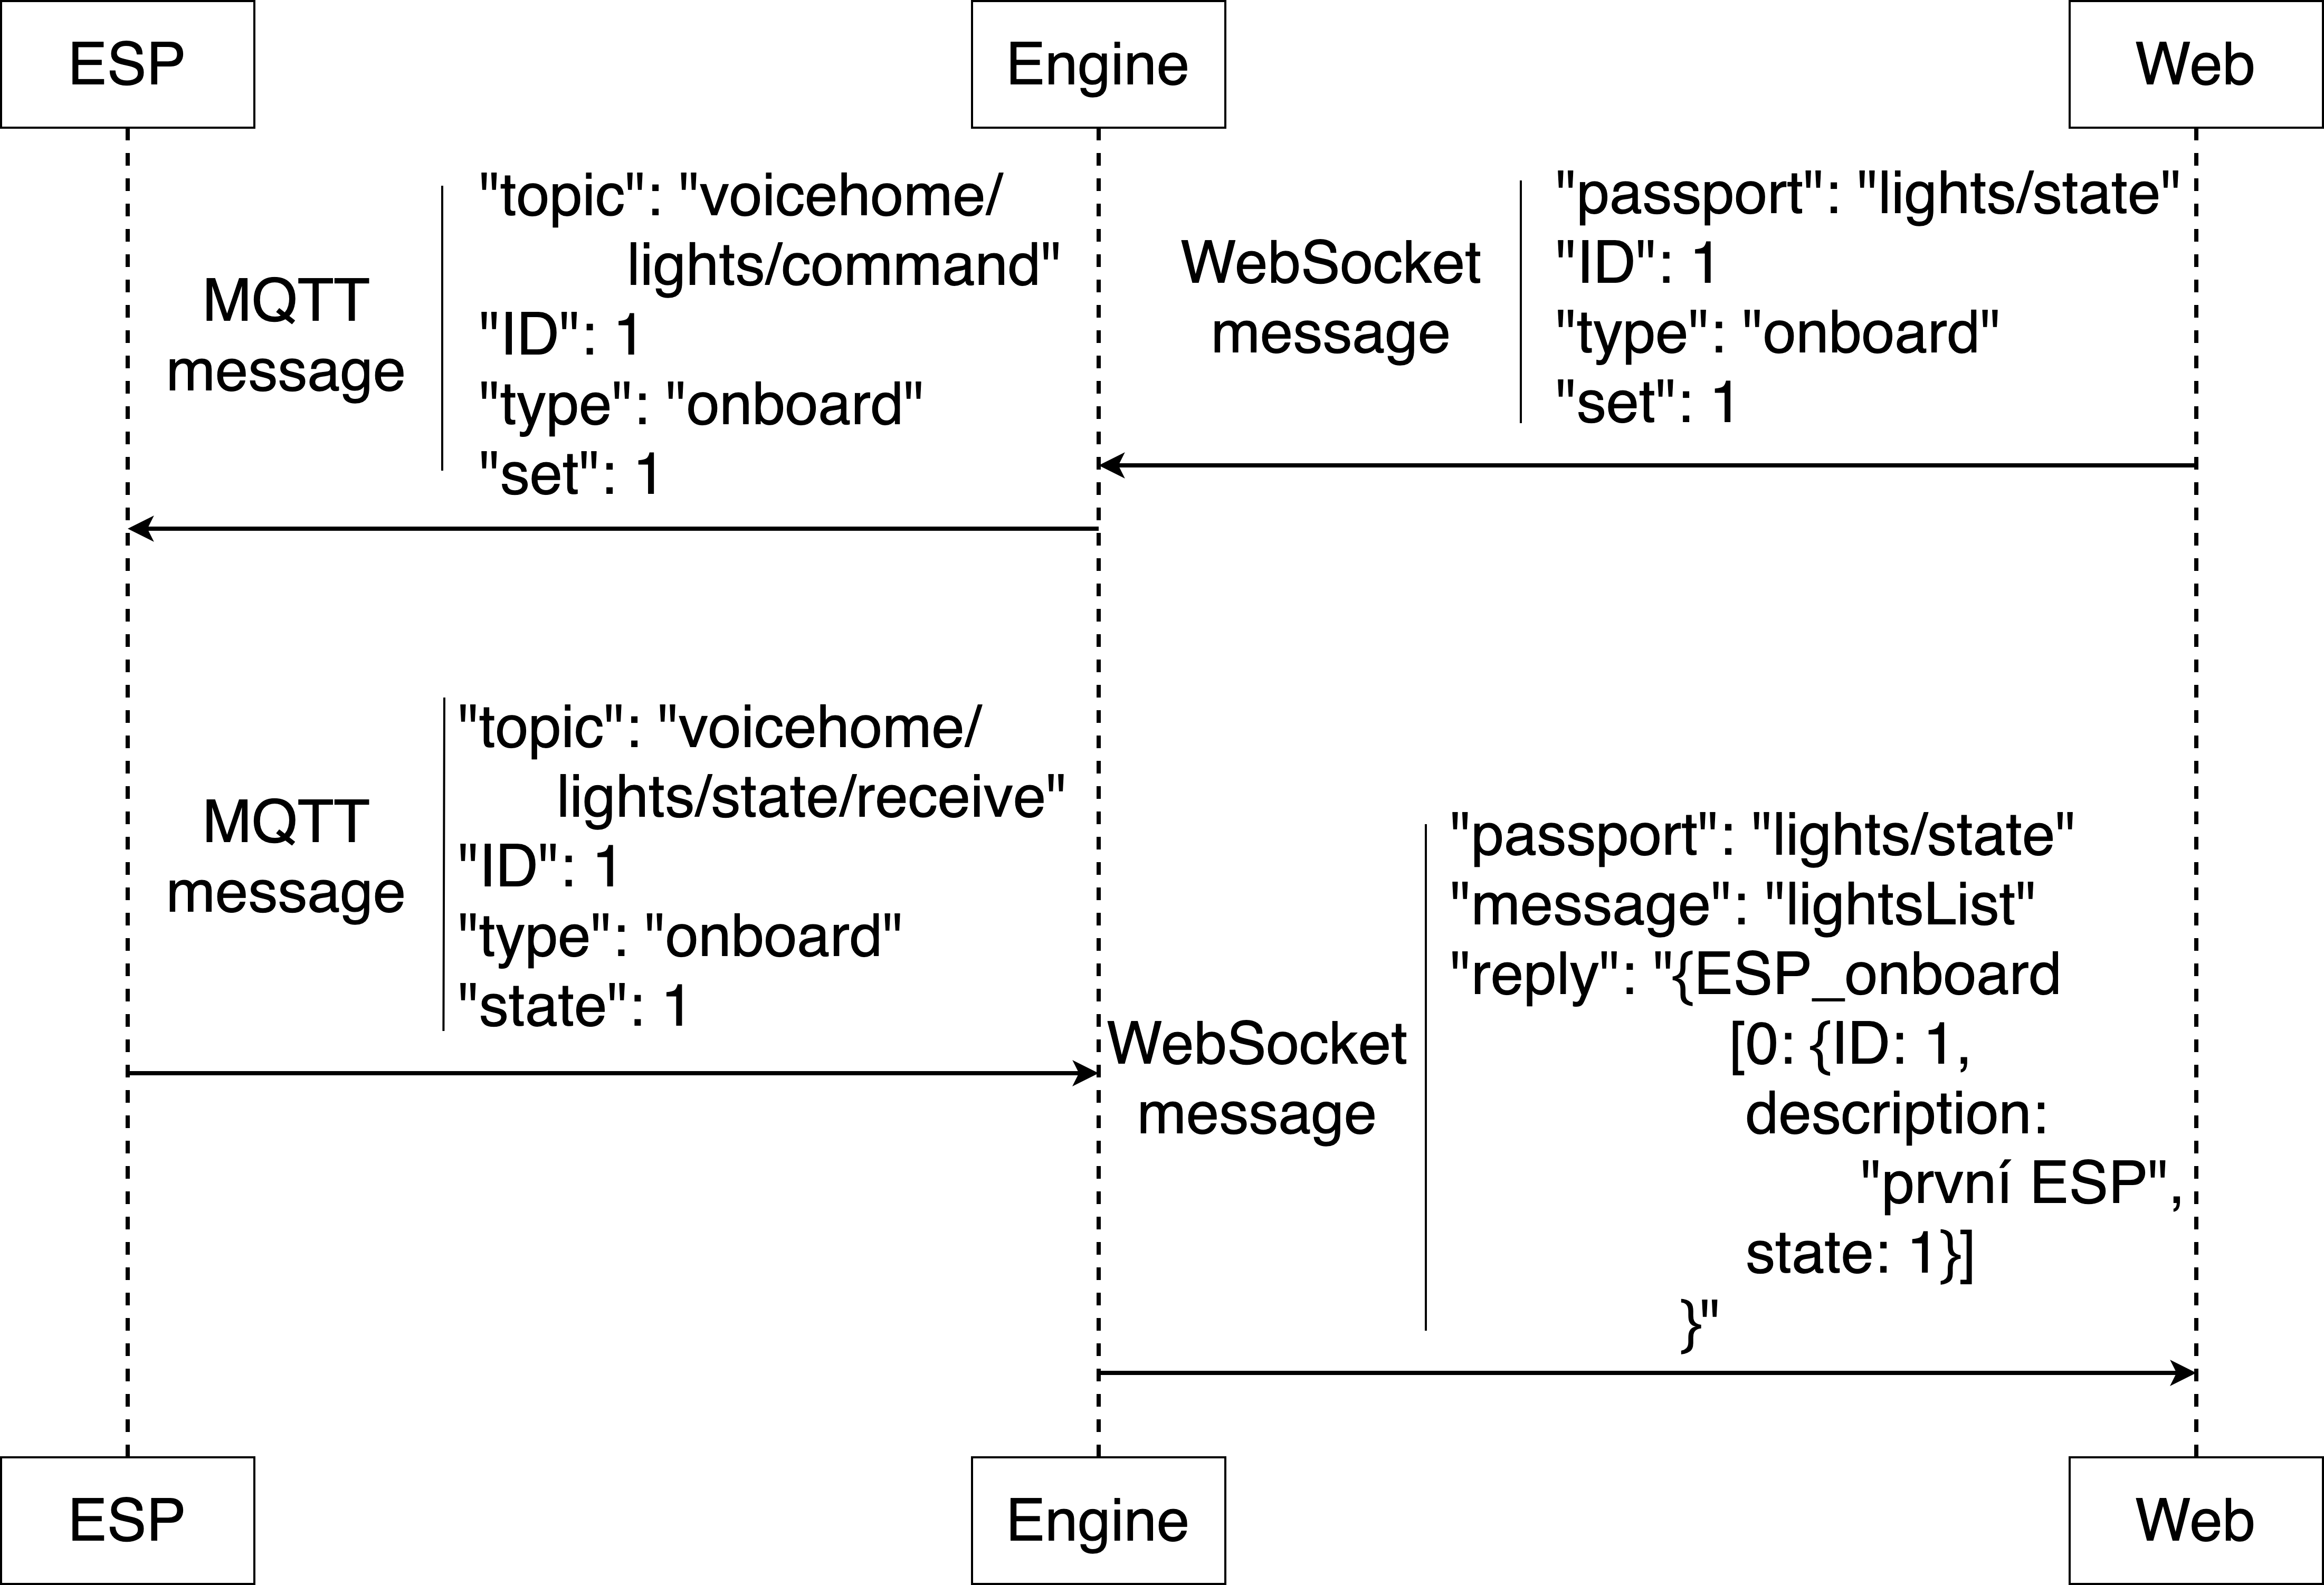
\includegraphics[width=\textwidth]{img/lights_onoff_messages.png}
	\caption{Diagram of message flows to turn on/off led on ESP by the website.}
	\label{fig:lights_onoff_messages}
\end{figure}
